\chapter{Strategy} \label{strategy}
\section{Stakeholders}
\begin{figure}[!ht]
  \centering
  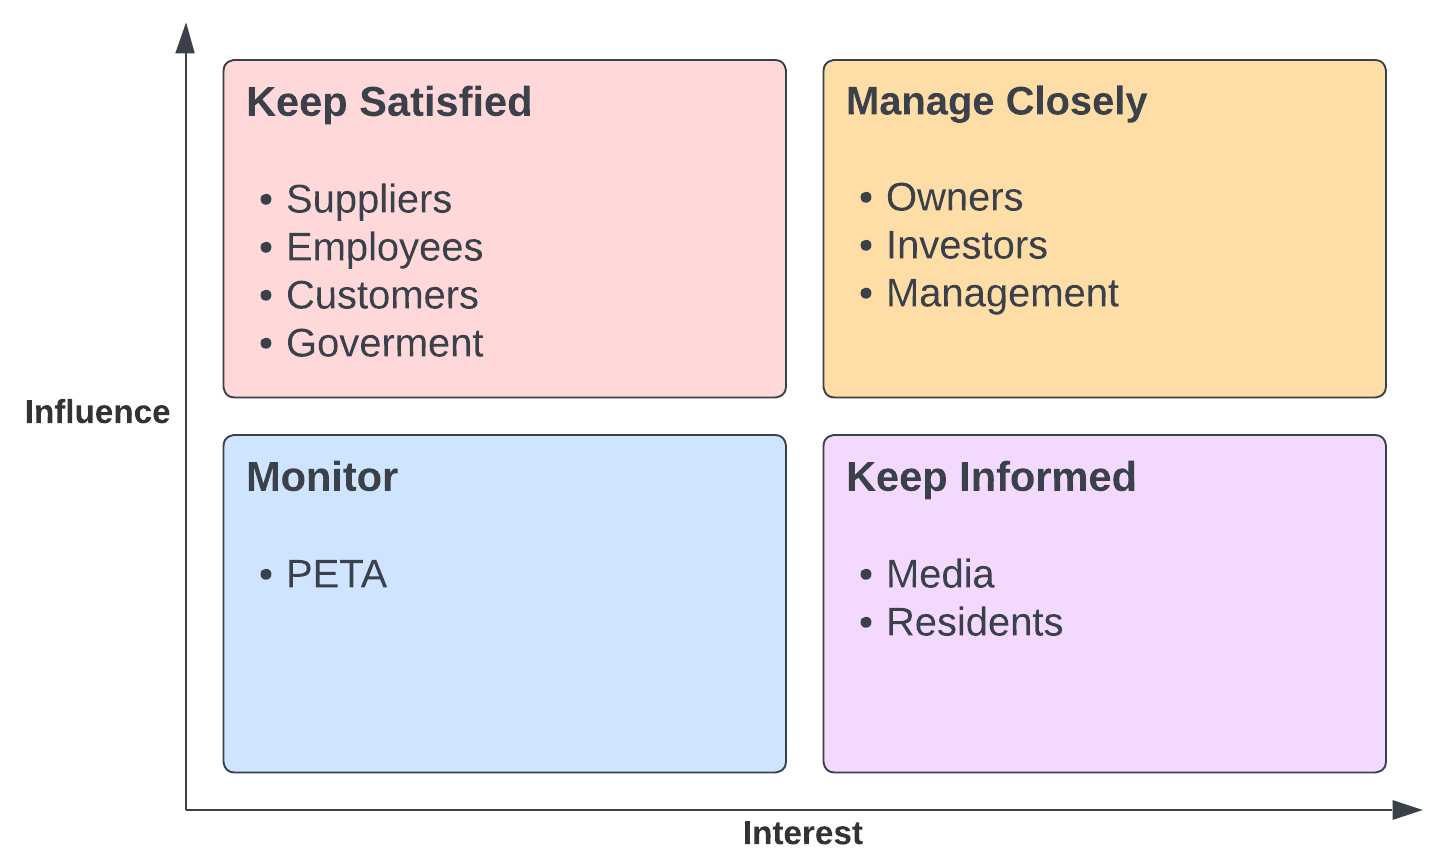
\includegraphics[width=0.8\linewidth]{./images/stakeholders.png}
  \caption[Stakeholder mapping made with lucidchart.com]{Diagram of the stakeholder mapping}
  \label{fig:stakeholders}
\end{figure}

\subsection{Internal}
We have various internal stakeholders. These include our employees in various areas, such as production or administration. The employees have an interest in the company because they want to protect their rights and secure their jobs so that they have a fixed income, fair working conditions, and can thus finance their livelihood.
\newline
Furthermore, we as owners are also internal stakeholders, as we want to make a profit from the money we invest. This also includes all other investors.
\newline
The management of the company is also one of our internal stakeholders; the management wants to achieve the company's goals in order to move it forward.
\subsection{External}
Our external stakeholders include the government, which is responsible for regulating the transportation of drones. But they also look at how our company works, whether we work according to all the guidelines.
\newline
Another external stakeholder are our customers (e.g., laboratories or hospitals), who use or would like to use our services and thus generate income. Then there are our shareholders, who want to make money with our shares.
\newline
Our suppliers are also very important external stakeholders, as they supply us with important materials for the construction of our drones. The society or the residents of the city in which we offer our service also play an essential role. For example, they can take action against us because they feel disturbed by the drones, which would not be good for our company image either. Groups such as \acs{peta} are also involved, as we operate in airspace and are therefore in a bird habitat. And last but not least, the media, it has a big impact on our company, whether the media writes good or bad things about us.
\section{\acs{swot}-analysis}
\subsection{Strengths}
\begin{itemize}
  \item It is an innovative solution that does not really exist at the moment.
  \item Our service has the potential to improve the efficiency and speed of transporting medical samples.
  \item Modern technology through self-flying drones, leads to fewer employees, which leads to cost savings.
\end{itemize}
\subsection{Weaknesses}
\begin{itemize}
  \item Autonomous flying of drones requires complex and good technology, leading to high costs due to development.
  \item Communication between the drones and the responsible employees must function smoothly.
  \item Technical failures of the drones.
\end{itemize}
\subsection{Opportunities}
\begin{itemize}
  \item Demand for medical services is increasing.
  \item In situations, such as COVID-19, medical samples could be transported very quickly. Costs could be saved thanks to the faster transportation route.
  \item Cooperation with hospitals and laboratories can facilitate access to the market.
\end{itemize}
\subsection{Threats}
\begin{itemize}
  \item Other companies entering or operating in this sector (transportation companies).
  \item The strict regulations on drone transportation of medical samples.
  \item Accidents with drones.
\end{itemize}
\subsection{SO Strategies}
\begin{itemize}
  \item As the demand for medical samples is increasing, we can convince and win customers with our faster and more efficient method of transporting medical samples.
  \item In crisis situations we can be very supportive as we can transport very quickly and easily. We could also gain a leading position.
  \item With our modern and good technology, we can gain new customers.
\end{itemize}
\subsection{ST Strategies}
\begin{itemize}
  \item With our unique technology, we can be better than other companies. We also want to patent our drone technology.
  \item Since we have very safe drones that also register when something is in front of them through a sensor, we can reduce accidents to a minimum.
\end{itemize}
\subsection{WO Strategies}
\begin{itemize}
  \item The high demand for transportation of medical samples enables us to cover our high development costs from the start.
  \item Our well-developed technology enables us to reduce technical failures to a minimum.
\end{itemize}
\subsection{WT Strategies}
\begin{itemize}
  \item Since it requires high costs to develop this technology, we assume that many other companies will not do this easily.
\end{itemize}
\section{Possible barriers of entry}
As we are developing our own drone, this can lead to high costs in the beginning. However, we want to solve this by getting investors, because we are convinced that once we have overcome the first phase of our start-up, we will take a leading position in this market. We want to assure our potential investors of our innovative ideas and technologies. We also want to gain new customers. Also, we want to retain them with reliable and competent service. In the best-case scenario, these customers will also recommend us to others.
\newline
It could also be difficult to obtain the necessary permits in the city for the transportation of medical samples using drones. But we want to change this by lobbying the government with our very safe technology. And also show them the many advantages of our idea (fast and cost-effective transportation in the medical field).
